
\section*{Introduction}

Monitoring is a crucial task for network operations. It is needed to ensure that all resources operate correctly (e.g., no
failures) and their configuration meets operator’s expectations (no congestion, required quality of service, etc.). Effective
monitoring is also fundamental for management tasks like traffic engineering, maintenance and troubleshooting.

\begin{figure}
\begin{center}
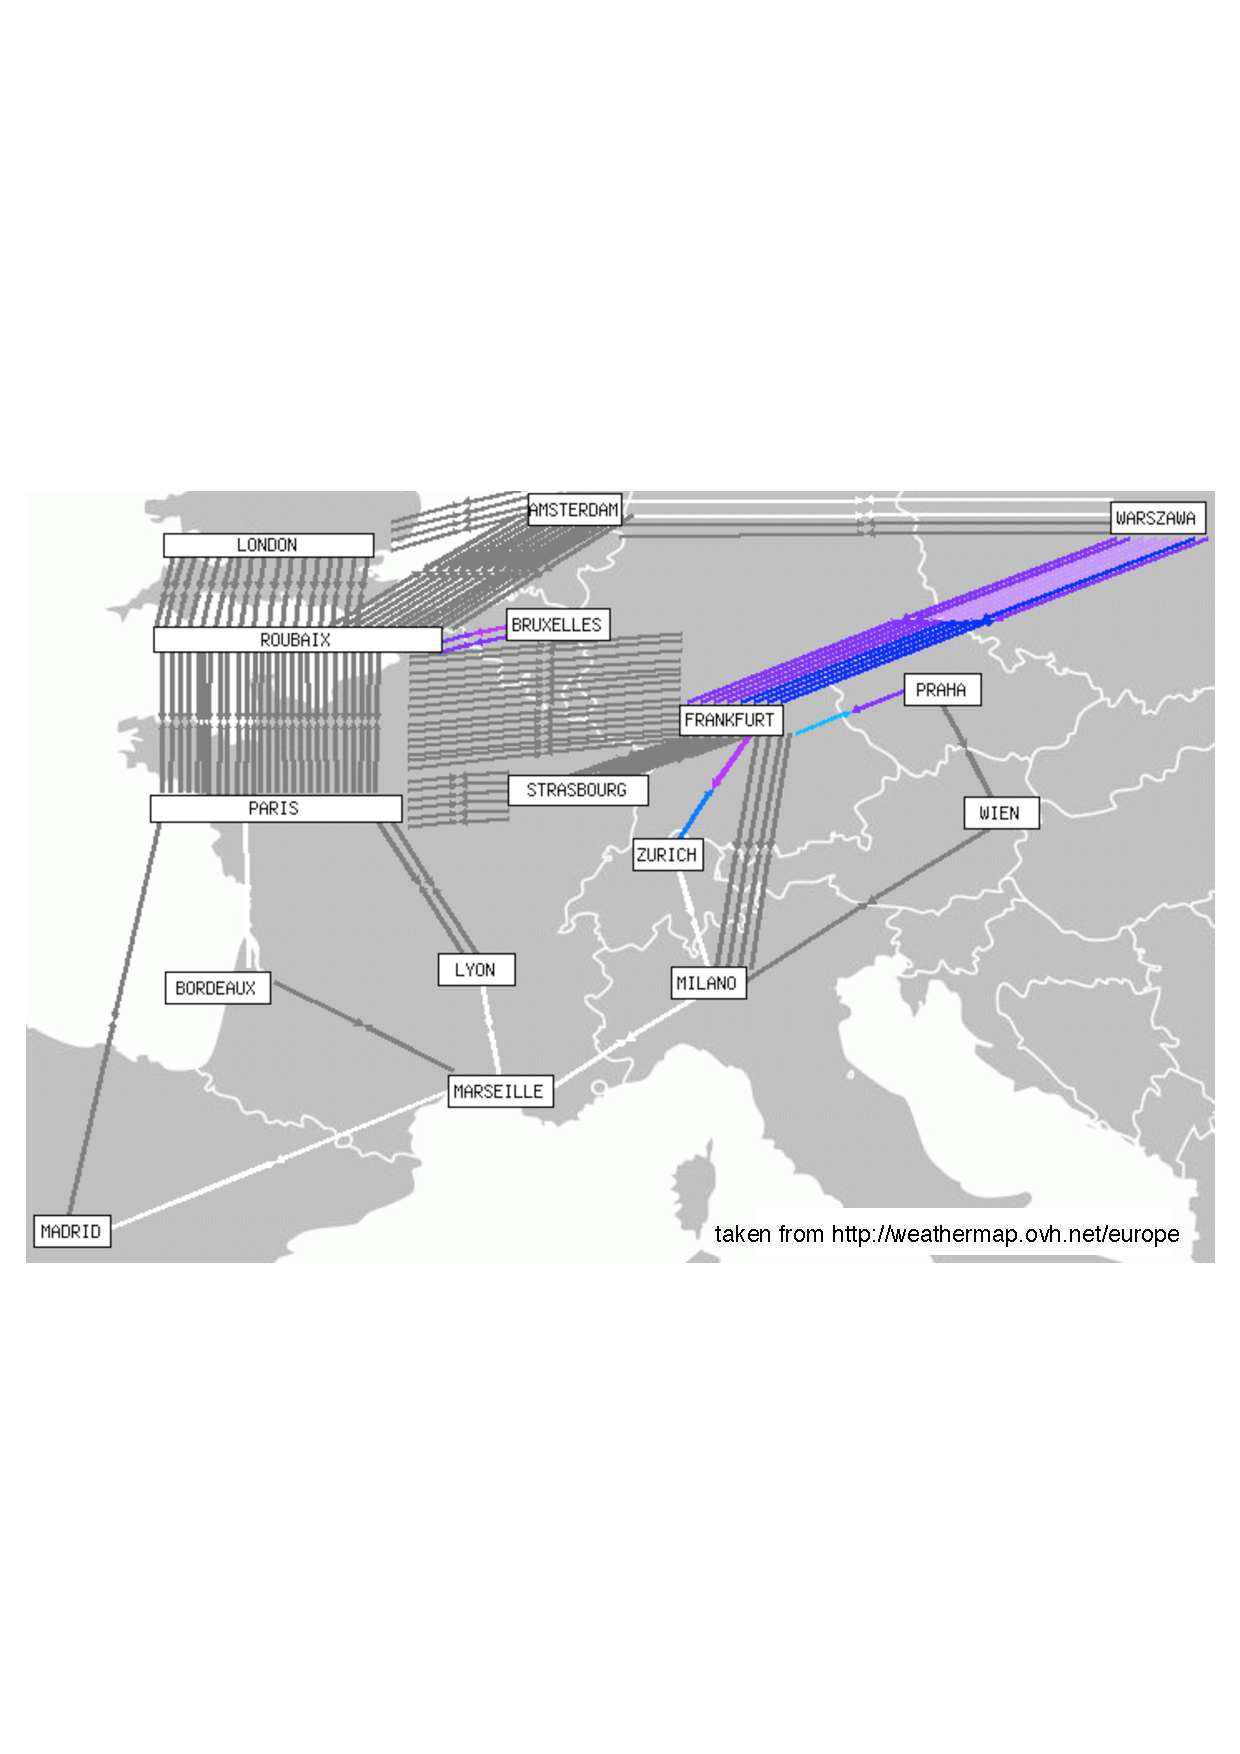
\includegraphics[width=.85\columnwidth]{figures/ovh-eu.pdf}
\end{center}
\caption{European backbone of \textsf{OVH}. In contrast to prior techniques, our algorithm can monitor health and performance of single
links in bundles (e.g., between \textsf{LONDON} and \textsf{ROUBAIX}).}
\label{fig:ovh}
\end{figure}


Unfortunately, even basic monitoring tasks, like checking for hardware malfunctions, are practically hard, due to the
complexity of current networks. Prominently, multi-path routing is widely used, both to spread the load on multiple paths
and to aggregate parallel links in bundles.
Figure \ref{fig:ovh} shows an overview of the European backbone of a big cloud provider,
\textsf{OVH}. It highlights that parallel links are used at the same time between many pairs of routers. While enabling better
performance and robustness, multi-path routing also poses significant obstacles to monitoring. For instance, assessing
the exact path and performance of each packet becomes complex [2], [20] since such a path depends on (vendor-specific) hash functions used by routers for load-balancing.

As a consequence, not only naive approaches (e.g., based on ping or traceroute) are not sufficient, but also 
state-of-the-art monitoring techniques tend to be ineffective.


On the one hand, protocol-based approaches use control-plane messages to infer possible failures. 
For example, link-state routing protocols (like OSPF or IS-IS) or specialized
ones (BFD [14]) rely on heartbeat-like mechanisms to check
bi-directional connectivity among pairs of adjacent nodes. This
approach only ensures detection of failures that affect control plane messages. 
However, it cannot be used to detect failures that only affect data-plane traffic like: 

\begin{enumerate}[i)]
\item corruption of an
optical link that leads to framing errors and packet losses;
\item malfunctioning of a router interface that considers the link still up but discards all the received packets;
\item failure of only one link among the parallel ones between two routers.
\end{enumerate}

On the other hand, probe-based techniques rely on sending
data-plane monitoring packets, i.e., probes, between fixed
vantage points in the network. Vantage points typically run
standard protocols (e.g., IPSLA [8]) to send probes and extract
measurements from them. Unfortunately, if the probes are sent
over paths used to forward regular traffic, many vantage points
may be needed to obtain high coverage, and links not used
by current paths (e.g., backup links) cannot be checked at
all. Otherwise, probes can be sent over tunnels (e.g., RSVP-TE [3] ones) to enforce specific paths, but this is not scalable.
Indeed, even for detecting single-link failures and pinpointing
their position, the number of needed tunnels tends to explode,
and so does the control-plane overhead (to signal tunnels) [7].

We propose a new technique that ensures full coverage of all network resources from a
single vantage point. It is based on sending data-plane probes over carefully-chosen cycles. This way, a single box can both
send and receive monitoring probes, avoiding the need for synchronizing and coordinating multiple vantage points, hence
minimizing infrastructural costs. By relying on data-plane measurements, we support both detection of hardware failures and resource overloading (e.g., link congestion).

% Segment routing generates conflicting objectives for the computation
% of cycles over which probes are sent. On the one hand, we would like to minimize the number of cycles, to reduce the
% monitoring overhead; hence, we should have cycles that are long and few in number. On the other hand, we need cycles
% to be enforced in practice, and long cycles may require too many segments even for the most powerful commercial routers
% (currently supporting less than 10 segments). To tackle those challenges, SCMon runs original algorithms
% that compute cycles on a monitoring topology, maintained by routers in addition to the one used for user traffic. The monitoring topology spans all network links, 
% and uses carefully computed weights that avoid (as much as possible) ECMP paths, i.e., multiple shortest paths between a pair of nodes.
% Note that existing routers have already been shown to well support two topologies and their (limited) overhead [17].
% SCMon supports detection and localization of any set of link failures/overloading. It infers single-link failures by keeping
% track of the cycles associated to probes sent and not received at the monitoring box. For multiple link failures, we have two
% cases. Some of them, e.g., affecting links in disjoint cycles, are detected directly from the set of lost probes (as single-link failures). 
% The others, e.g., affecting two links belonging to a single monitoring cycle, are reported by SCMon one at
% a time: This provides operators with a debugging interface (asking to correct one error before showing another one)
% similar to the one of a compiler for software programs. Similar considerations apply to node failures and link congestion.
% In developing SCMon, we make three main contributions.
% 
% Our approach to compute monitoring cycles consists of four steps.
% The first step computes IGP weights for the monitoring topology, in order to minimize ECMP paths.
% The second step models link bundles aggregated into a single IGP link. 
% The third step calculates a set of cycles covering the whole network and sharing the node from which probes are sent.
% The last step computes the SR segments to send probes over those cycles.


%In this section we will propose several algorithms and strategies to compute a cycle cover of the network
%using segment routing. We need however to impose some properties in the cycle cover in order to be able to use
%it for detecting single link failures in a network. Those properties as the following:

As usual, we start by defining the problems that we tackle in this chapter. To do that we need the two following definitions.
Throughout this chapter we assume that the network topology is symmetric.

\begin{definition}
Let $G$ be a symmetric network, $s \in V(G)$ and $k \in \mathbb{N}$. We denote by $\mathcal{C}^k_s$ the set of deterministic sr-cycles from $s$ to $s$ with segment cost at most $k$.
\end{definition}

\begin{definition}
Let $G$ be a symmetric network, $s \in V(G)$ and $k \in \mathbb{N}$. A \emph{$k$ sr-cycle cover} of a network $G$ 
with vantage point $s$ is a subset $C \subseteq \mathcal{C}^k_s$ of deterministic sr-cycles such
that for each edge $e \in E(G)$ there exists $\sr{c} \in C$ such that $e \in E(\sr{c})$.
\end{definition}

Below we define the two problems that we tackle in this chapter. Both of them seek to compute a cycle cover.
The first aims at minimizing the maximum segment cost of any sr-cycle in the cover while the second wants to minimize the number of cycles for a given segment cost limit.
% We will see that the first problem admits a polynomial time solution and that the second one is \NPhard.


\begin{problem}{Min segment cost cover}
\label{prob:min-seg-cover}
\textbf{Input:} A symmetric network $G$ and $s \in V(G)$.

\textbf{Output:} A sr-cycle cover $C$ of $G$ such that the maximum segment cost of any sr-cycle $\sr{c} \in C$ is minimum.
\end{problem}

\begin{problem}{Min sr-cycle cover}
\label{prob:min-cycle-cover}
\textbf{Input:} A symmetric network $G$, $s \in V(G)$ and $k \in \mathbb{N}$.

\textbf{Output:} A sr-cycle cover $C \subseteq \Csk$ of $G$ such that $|C|$ is minimum.
\end{problem}
% 
% \begin{proposition}
% Problem \ref{prob:min-cycle-cover} is \NPhard.
% \end{proposition}
% 
% \begin{proof}
% The problem of finding a minimum cardinaly cycle cover of a graph is \NPhard and by setting $k$
% large enough and setting IGP weights such that there is not ECMP any solution
% to Problem \ref{prob:min-cycle-cover} corresponds to a minimum cycle cover.
% \end{proof}
% 
